\section{Checking without knowing the future}\label{sec:online}

The schedules of Sections~\ref{sec:entropy} to~\ref{sec:singularity} are computed from the whole cost profile: the number of runs of the $i$-th check depends on $A$ and on every other cost. A self-improving system does not know its future modifications. When the $n$-th candidate arrives, only $a_{1},\dots,a_{n}$ are known, and the number of runs of its check must be fixed then. This section shows that such a system loses almost nothing: the entropy law survives with an additive term that grows like the logarithm of the logarithm of the dynamic range, and that term cannot be removed.

\subsection{Online schedules}

An \emph{online schedule} is a rule that assigns to each finite sequence $(a_{1},\dots,a_{n})$ of positive costs a number $r_{n}\in\NN$ of runs for the last candidate. Applied to a sequence $(a_{n})_{n\ge1}$, finite or infinite, it produces the schedule $(r_{n})$, and $r_{n}$ does not depend on $a_{n+1},a_{n+2},\dots$. The rule is \emph{$\theta$-sound} if $\sum_{n}\eps^{r_{n}}\le\theta$ for every sequence of positive costs. Write
\[
S_{n}=a_{1}+\dots+a_{n},\qquad u_{n}=\log\frac{S_{n}}{a_{1}},\qquad w_{n}=\frac{a_{n}/S_{n}}{2(1+u_{n})^{2}},
\]
so that $u_{1}=0$, $u_{n}$ is nondecreasing and $w_{1}=\frac12$. On the first $N$ candidates write $A_{N}=S_{N}$, $p^{(N)}=(a_{n}/A_{N})_{n\le N}$, $V_{N}=\sum_{n\le N}a_{n}r_{n}$ and $\Vs_{N}(\theta)$ for the offline optimum of Theorem~\ref{thm:A}.

\begin{mainthm}[Online entropy law]\label{thm:G}
Let $0<\eps<1$ and $0<\theta\le1$. The online schedule
\begin{equation}\label{eq:onlinerule}
r_{n}=\Bigl\lceil\frac1L\log\frac{1}{\theta w_{n}}\Bigr\rceil=\Bigl\lceil\frac1L\log\frac{2(1+u_{n})^{2}S_{n}}{\theta a_{n}}\Bigr\rceil
\end{equation}
is $\theta$-sound, and for every $N$
\begin{equation}\label{eq:onlineupper}
V_{N}\le\frac{A_{N}}{L}\Bigl(H(p^{(N)})+\log\frac1\theta+\log2+2\log\Bigl(1+\log\frac{A_{N}}{a_{1}}\Bigr)\Bigr)+A_{N}.
\end{equation}
Conversely, on the doubling costs $a_{n}=2^{n-1}$ every $\theta$-sound online schedule satisfies, for infinitely many $N$,
\begin{equation}\label{eq:onlinelower}
V_{N}-\Vs_{N}(\theta)\ \ge\ \frac{A_{N}}{2L}\log\log_{2}\Bigl(1+\frac{A_{N}}{a_{1}}\Bigr)-\Bigl(1+\frac{2\log2}{L}\Bigr)A_{N}.
\end{equation}
\end{mainthm}

Together with the lower bound of Theorem~\ref{thm:A}, \eqref{eq:onlineupper} says that the price of not knowing the future is at most $(A_{N}/L)(\log2+2\log(1+\log(A_{N}/a_{1})))+A_{N}$, and \eqref{eq:onlinelower} says that a term of order $(A_{N}/L)\log\log(A_{N}/a_{1})$ must be paid by every online rule on some sequences. The two bounds differ by a factor of four in the leading term. The dynamic range $A_{N}/a_{1}$ enters only through a double logarithm: a system whose total checking cost grows by a factor $10^{100}$ over its first candidate pays at most $2\log(1+100\log10)\approx10.9$ extra runs per unit of cost, measured in units of $L$.

\begin{corollary}[Sound singularities without foresight]\label{cor:onlinesing}
If $\sum_{n}a_{n}<\infty$ and $\sum_{n}a_{n}\log(1/a_{n})<\infty$, the online schedule \eqref{eq:onlinerule} is $\theta$-sound and has finite total cost
\[
V\le\frac{A}{L}\Bigl(H(p)+\log\frac1\theta+\log2+2\log\Bigl(1+\log\frac{A}{a_{1}}\Bigr)\Bigr)+A .
\]
\end{corollary}

So the criterion of Theorem~\ref{thm:E} does not need an oracle. A chain that only knows its past costs reaches a sound singularity whenever any chain does, and the rule that achieves it is the same for every sequence.

\subsection{Proofs}

The proof rests on two elementary facts, both proved in Lean (Appendix~\ref{app:checks}).

\begin{lemma}[Telescoping]\label{lem:telescope}
For $0\le x\le y$, $\dfrac{y-x}{(1+y)^{2}}\le\dfrac1{1+x}-\dfrac1{1+y}$. Hence for a nondecreasing sequence $0\le u_{1}\le u_{2}\le\cdots$,
\[
\sum_{n=2}^{N}\frac{u_{n}-u_{n-1}}{(1+u_{n})^{2}}\ \le\ \frac1{1+u_{1}}-\frac1{1+u_{N}}.
\]
\end{lemma}

\begin{proof}
The right side of the first inequality is $(y-x)/((1+x)(1+y))$, and $(1+x)\le(1+y)$. Summing gives a telescoping series.
\end{proof}

\begin{lemma}[Share of the newest cost]\label{lem:share}
For $0<s\le t$, $1-s/t\le\log(t/s)$. In particular $a_{n}/S_{n}=1-S_{n-1}/S_{n}\le u_{n}-u_{n-1}$ for $n\ge2$.
\end{lemma}

\begin{proof}
This is $1-1/x\le\log x$ at $x=t/s$, which is $\log y\le y-1$ at $y=1/x$. For the second statement take $s=S_{n-1}$, $t=S_{n}$ and note $\log(S_{n}/S_{n-1})=u_{n}-u_{n-1}$.
\end{proof}

\begin{proof}[Proof of Theorem~\ref{thm:G}]
\emph{Soundness.} By Lemma~\ref{lem:share} and Lemma~\ref{lem:telescope},
\[
\sum_{n=1}^{N}w_{n}=\frac12+\frac12\sum_{n=2}^{N}\frac{a_{n}/S_{n}}{(1+u_{n})^{2}}\le\frac12+\frac12\sum_{n=2}^{N}\frac{u_{n}-u_{n-1}}{(1+u_{n})^{2}}\le\frac12+\frac12\Bigl(1-\frac1{1+u_{N}}\Bigr)<1
\]
for every $N$ and every sequence of positive costs. Since $w_{n}\le\frac12<1$ and $\theta\le1$, the number inside the ceiling of \eqref{eq:onlinerule} is positive and $\eps^{r_{n}}\le\theta w_{n}$. Hence $\sum_{n}\eps^{r_{n}}\le\theta\sum_{n}w_{n}\le\theta$, and $r_{n}$ depends only on $a_{1},\dots,a_{n}$.

\emph{Cost.} From $r_{n}<\frac1L\log\frac1{\theta w_{n}}+1$,
\[
L\,V_{N}<\sum_{n\le N}a_{n}\Bigl(\log\frac1\theta+\log2+2\log(1+u_{n})+\log\frac{S_{n}}{a_{n}}\Bigr)+L\,A_{N}.
\]
For $n\le N$ we have $S_{n}\le A_{N}$, so $\log(S_{n}/a_{n})\le\log(A_{N}/a_{n})$ and $u_{n}\le\log(A_{N}/a_{1})$. Since $\sum_{n\le N}a_{n}\log(A_{N}/a_{n})=A_{N}H(p^{(N)})$, \eqref{eq:onlineupper} follows.

\emph{Lower bound.} Fix a $\theta$-sound online rule and apply it to the infinite sequence $a_{n}=2^{n-1}$. Its decisions on the first $N$ candidates are those it takes on the finite sequence $(a_{1},\dots,a_{N})$. Put $v_{n}=\eps^{r_{n}}/\theta$, so $\sum_{n}v_{n}\le1$. Then $v_{N}\le1/N$ for infinitely many $N$: otherwise $v_{N}>1/N$ for all large $N$ and $\sum v_{N}$ would diverge with the harmonic series. For such $N$, $r_{N}L\ge\log(N/\theta)$, and $r_{n}L\ge\log(1/\theta)$ for every $n$ because $\eps^{r_{n}}\le\theta$. Hence
\[
L\,V_{N}\ \ge\ A_{N}\log\frac1\theta+a_{N}\log N .
\]
On the other side, $p^{(N)}_{n}=2^{n-1}/(2^{N}-1)\ge2^{n-1-N}$, so
\[
H(p^{(N)})\le\log2\sum_{n=1}^{N}(N-n+1)\,p^{(N)}_{n}=\log2\cdot\frac{2^{N+1}-N-2}{2^{N}-1}\le2\log2,
\]
by the identity $\sum_{k=1}^{N}k2^{-k}=2-(N+2)2^{-N}$, and Theorem~\ref{thm:A} gives $L\,\Vs_{N}(\theta)\le A_{N}(2\log2+\log\frac1\theta)+LA_{N}$. Subtracting, and using $a_{N}=2^{N-1}\ge A_{N}/2$ and $N=\log_{2}(1+A_{N}/a_{1})$, gives \eqref{eq:onlinelower}.
\end{proof}

\begin{proof}[Proof of Corollary~\ref{cor:onlinesing}]
Soundness is that of Theorem~\ref{thm:G}. For the cost, the argument of the upper bound with $A$ in place of $A_{N}$ bounds every partial sum $V_{N}$ by the right side, since $S_{n}\le A$ for all $n$ and $\sum_{n\le N}a_{n}\log(A/a_{n})\le AH(p)$. The right side is finite because $AH(p)=A\log A+\sum_{n}a_{n}\log(1/a_{n})$.
\end{proof}

\subsection{Universal codes}

Theorem~\ref{thm:G} is the schedule counterpart of the universal codes for the integers. Elias constructed prefix codes whose length for the integer $m$ is $\log m+O(\log\log m)$ without knowledge of the distribution of $m$ \cite{Eli75}, and Rissanen derived from them a universal prior whose code length $\log^{\ast}m$ is optimal up to the iterated logarithms \cite{Ris83}. Here the role of the integer is played by the ratio $S_{n}/a_{1}$, the weight $w_{n}$ is a code length in disguise, and the double logarithm of \eqref{eq:onlineupper} is the price of the second level of the Elias code. The constant $2$ in front of it can be lowered to $1+\delta$ for every $\delta>0$ by replacing $(1+u_{n})^{2}$ with $c_{\delta}(1+u_{n})(1+\log(1+u_{n}))^{1+\delta}$, as in the Elias $\omega$ code; the lower bound \eqref{eq:onlinelower} shows that no rule removes the double logarithm.

Figure~\ref{fig:online} shows the rule at work. On random profiles its cost stays within the band of Theorem~\ref{thm:G}, and on the doubling sequence the excess over the offline optimum grows like $\log\log$ of the dynamic range, as the lower bound requires.

\begin{figure*}[t]
\centering
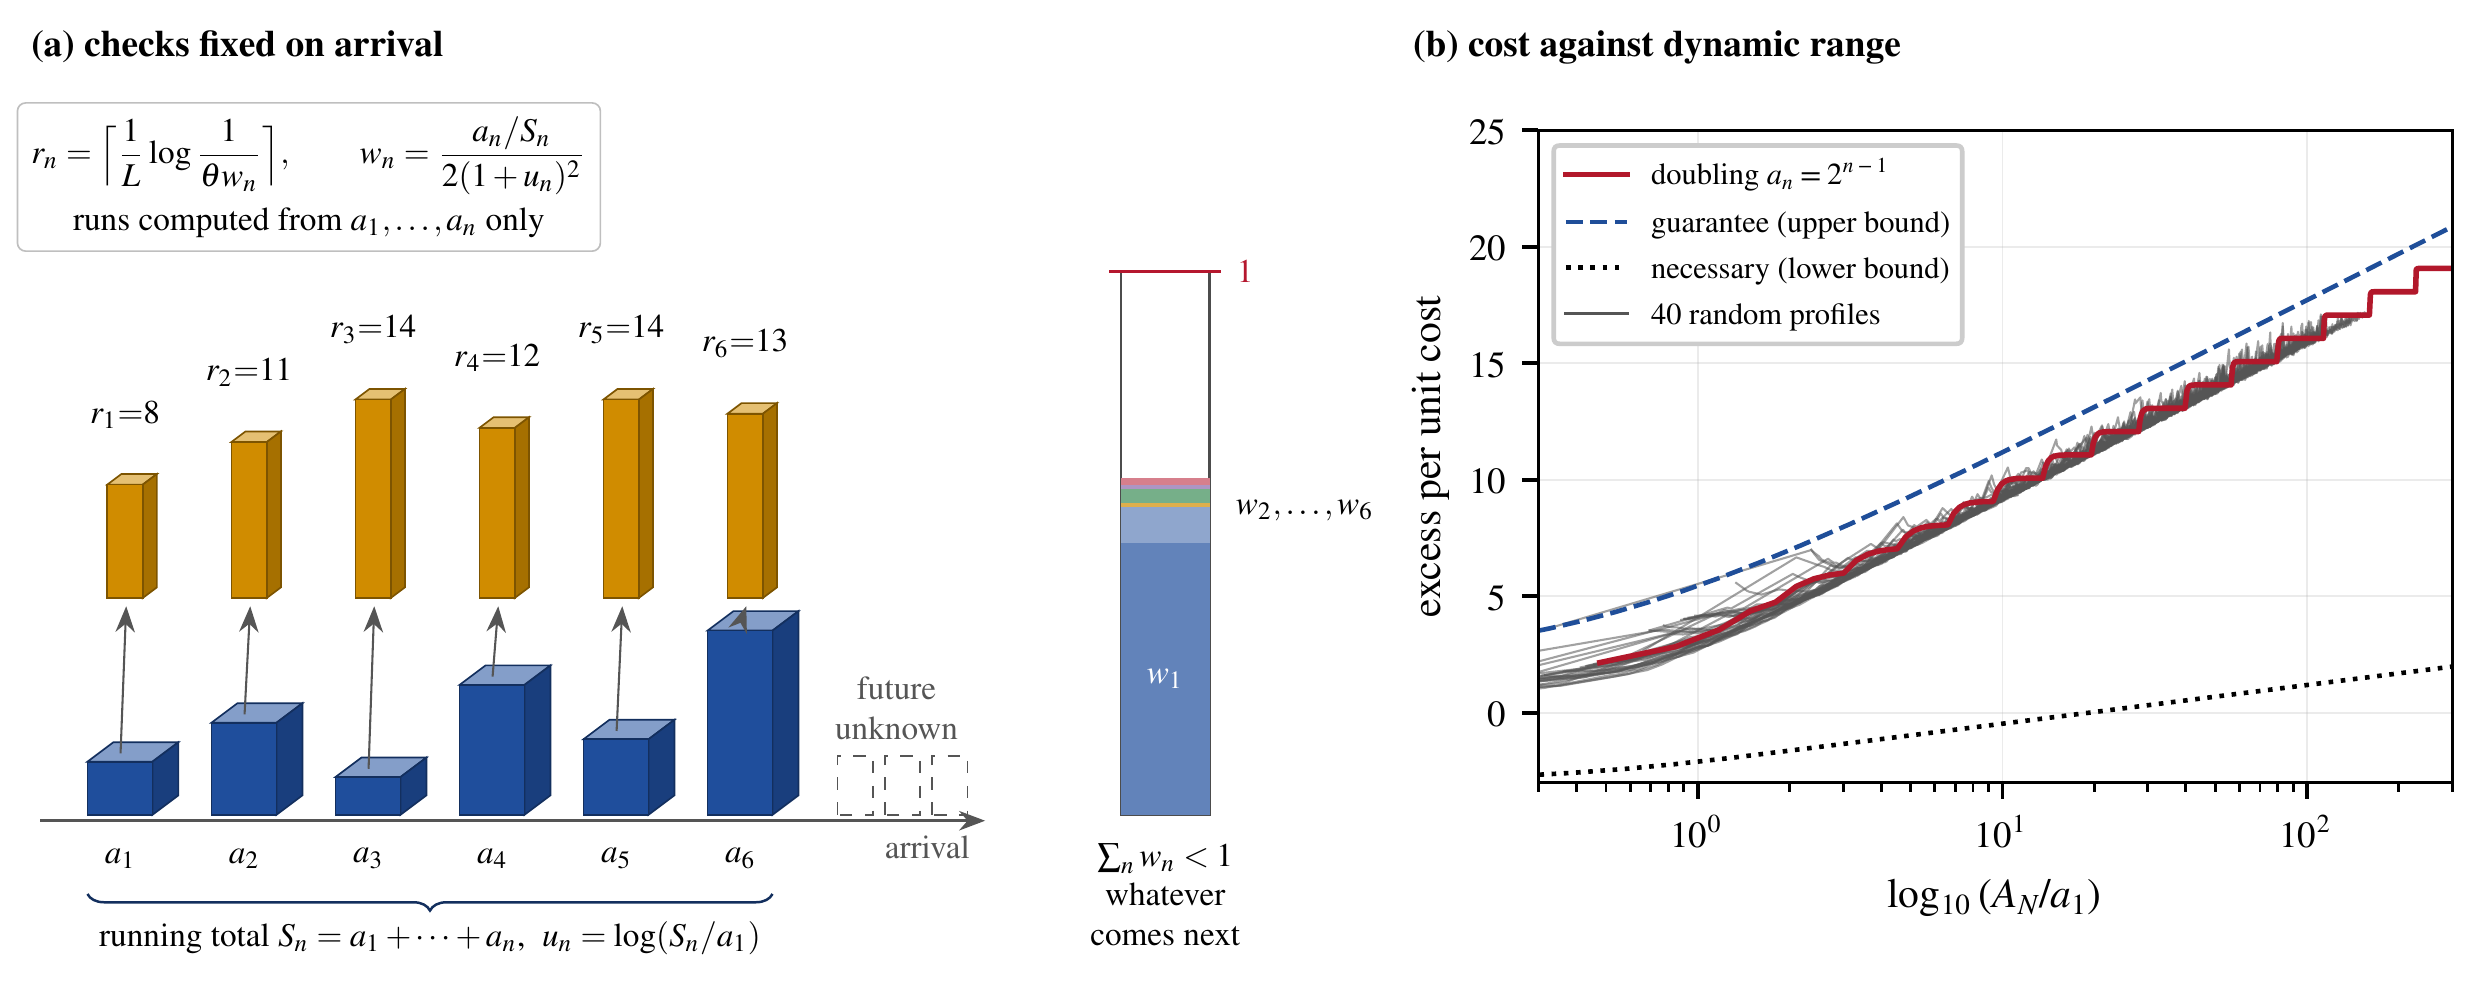
\includegraphics[width=0.98\textwidth]{figures/fig_online}
\caption{The online entropy law. (a) Candidates arrive one at a time; the $n$-th check is given $r_{n}$ runs computed from the running total $S_{n}$ alone, and the weights $w_{n}$ never sum to more than one, whatever comes next. (b) The excess $(V_{N}-\frac{A_{N}}{L}(H+\log\frac1\theta))/A_{N}$ of the online rule over the offline lower bound, for the doubling sequence $a_{n}=2^{n-1}$ (red) and for forty random profiles with log-normal costs (grey), against $\log_{10}(A_{N}/a_{1})$, with $\eps=\frac12$ and $\theta=10^{-6}$. The dashed curve is the guarantee $(\log2+2\log(1+\log(A_{N}/a_{1})))/L+1$ of \eqref{eq:onlineupper}, and the dotted curve is the necessary excess $\frac1{2L}\log\log_{2}(1+A_{N}/a_{1})-1-\frac{2\log2}{L}$ of \eqref{eq:onlinelower}.}
\label{fig:online}
\end{figure*}
